\documentclass[25pt, a0paper, portrait]{tikzposter}
% \documentclass{tikzposter}
% \geometry{paperwidth=36in,paperheight=44in}
\makeatletter
\setlength{\TP@visibletextwidth}{\textwidth-2\TP@innermargin}
\setlength{\TP@visibletextheight}{\textheight-2\TP@innermargin}
\makeatother


\makeatletter
\newcommand\insertlogoi[2][]{\def\@insertlogoi{\includegraphics[#1]{#2}}}
\newcommand\insertlogoii[2][]{\def\@insertlogoii{\includegraphics[#1]{#2}}}
\newcommand{\tikzpar}{\setlength{\parindent}{5ex}}
\newlength\LogoSep
\setlength\LogoSep{-100pt}

\insertlogoi[width=10cm]{src/D-Pine.eps}
\insertlogoii[width=7cm]{src/CS21.png}
% \usetheme{Simple}

\newcounter{tablecounter}
\newenvironment{tikztable}[1][]{
  \def \rememberparameter{#1}
  \vspace{10pt}
  \refstepcounter{tablecounter}
  \begin{center}
  }{
    \ifx\rememberparameter\@empty
    \else
    \\[10pt]
    {\small Tab.~\thetablecounter: \rememberparameter}
    \fi
  \end{center}
}


\renewcommand\maketitle[1][]{  % #1 keys
    \normalsize
    \setkeys{title}{#1}
    % Title dummy to get title height
    \node[transparent,inner sep=\TP@titleinnersep, line width=\TP@titlelinewidth, anchor=north, minimum width=\TP@visibletextwidth-2\TP@titleinnersep]
        (TP@title) at ($(0, 0.5\textheight-\TP@titletotopverticalspace)$) {\parbox{\TP@titlewidth-2\TP@titleinnersep}{\TP@maketitle}};
    \draw let \p1 = ($(TP@title.north)-(TP@title.south)$) in node {
        \setlength{\TP@titleheight}{\y1}
        \setlength{\titleheight}{\y1}
        \global\TP@titleheight=\TP@titleheight
        \global\titleheight=\titleheight
    };

    % Compute title position
    \setlength{\titleposleft}{-0.5\titlewidth}
    \setlength{\titleposright}{\titleposleft+\titlewidth}
    \setlength{\titlepostop}{0.5\textheight-\TP@titletotopverticalspace}
    \setlength{\titleposbottom}{\titlepostop-\titleheight}

    % Title style (background)
    \TP@titlestyle

    % Title node
    \node[inner sep=\TP@titleinnersep, line width=\TP@titlelinewidth, anchor=north, minimum width=\TP@visibletextwidth-2\TP@titleinnersep]
        at (0,0.5\textheight-\TP@titletotopverticalspace)
        (title)
        {\parbox{\TP@titlewidth-2\TP@titleinnersep}{\TP@maketitle}};

    \node[inner sep=0pt,anchor=west] 
      at ([xshift=-\LogoSep]title.west)
      {\@insertlogoi};

    \node[inner sep=0pt,anchor=east] 
      at ([xshift=\LogoSep]title.east)
      {\@insertlogoii};

    % Settings for blocks
    \normalsize
    \setlength{\TP@blocktop}{\titleposbottom-\TP@titletoblockverticalspace}
}
\makeatother

\definecolorstyle{sampleColorStyle} {
	\definecolor{colorOne}{named}{white}
	\definecolor{colorTwo}{named}{red}
	\definecolor{colorThree}{named}{red}
	\definecolor{Dgreen}{HTML}{00693e}
}{
	% Background Colors
	\colorlet{backgroundcolor}{colorOne}
	\colorlet{framecolor}{white}
	% Title Colors
	\colorlet{titlefgcolor}{white}
	\colorlet{titlebgcolor}{Dgreen}
	% Block Colors
	\colorlet{blocktitlebgcolor}{white}
	\colorlet{blocktitlefgcolor}{Dgreen}
	\colorlet{blockbodybgcolor}{white}
	\colorlet{blockbodyfgcolor}{black}
	% Innerblock Colors
	\colorlet{innerblocktitlebgcolor}{white}
	\colorlet{innerblocktitlefgcolor}{black}
	\colorlet{innerblockbodybgcolor}{colorThree!30!white}
	\colorlet{innerblockbodyfgcolor}{black}
	% Note colors
	\colorlet{notefgcolor}{black}
	\colorlet{notebgcolor}{colorTwo!50!white}
	\colorlet{noteframecolor}{colorTwo}
}

\definelayouttheme{sample}{
	\usecolorstyle[colorPalette=sampleColorPalette]{sampleColorStyle}
	\usebackgroundstyle{sample}
	\usetitlestyle{Test}
	\useblockstyle{Simple}
	\useinnerblockstyle{Simple}
	\usenotestyle{Corner}
}

\usetheme{sample}

% \begin{document}
%\geometry{paperwidth=44in,paperheight=36in}
\usetitlestyle{Filled}
\title{
\begin{minipage}{\textwidth}
   \centering
   Updated High-Temperature Opacities for DSEP
   \\
   \bigskip
   \mbox{and their Effect on the Jao Gap Location}
 \end{minipage}
 }
% \title{Updated High-Temperature Opacities for The Dartmouth Stellar Evolution Program and their Effect on the Jao Gap Location}
\author{Thomas M. Boudreaux$^{1}$ \& Brian C. Chaboyer$^{1}$}
\institute{{Department of Physics and Astronomy, Dartmouth College, Hanover, NH 03755, USA}}
\usepackage[utf8]{inputenc}
\usepackage{wrapfig}
\usepackage{amsmath}
\usepackage{setspace}
\usepackage{fontspec}
\usepackage[T1]{fontenc}
\usepackage{adjustbox}
\usepackage{tikz}
\usepackage{xcolor}

\tikzposterlatexaffectionproofoff

\begin{document}
	\maketitle
	\begin{columns}
	    \column{0.33}
		\block{Abstract}{\fontsize{38}{45}\selectfont
			\tikzpar The Jao Gap (Jao et al. 2018), a 17 percent decrease in
			stellar density at $M_{G} \sim 10$ identified in both Gaia DR2 and
			EDR3 data, presents a new method to probe the interior structure of
			stars near the fully convective transition mass. The Gap is
			believed to originate from convective kissing instability wherein
			asymmetric production of 3He causes the core convective zone of a
			star to periodically expand and contract and consequently the
			stars’ luminosity to vary. Modeling of the Gap has revealed a
			sensitivity in its magnitude to a population’s metallicity and
			consequently opacity. Thus far, models of the Jao Gap have relied
			on OPAL high-temperature radiative opacities.  However, OPLIB
			opacities (Colgan et al. 2016) are more up to date. Use of these
			updated opacities changes the predicted location of the Jao Gap by
			~0.05 mag as compared to models which use the OPAL opacities. 

			\vspace{-25mm}
	    }
		\block{Updating Opacities}{\fontsize{38}{45}\selectfont
	    \vspace{-5mm}
			\begin{tikzfigure}[Solar Calibrated Stellar Models using both OPAL
				(black) and OPLIB (red) high--temperature opacity tables.]
				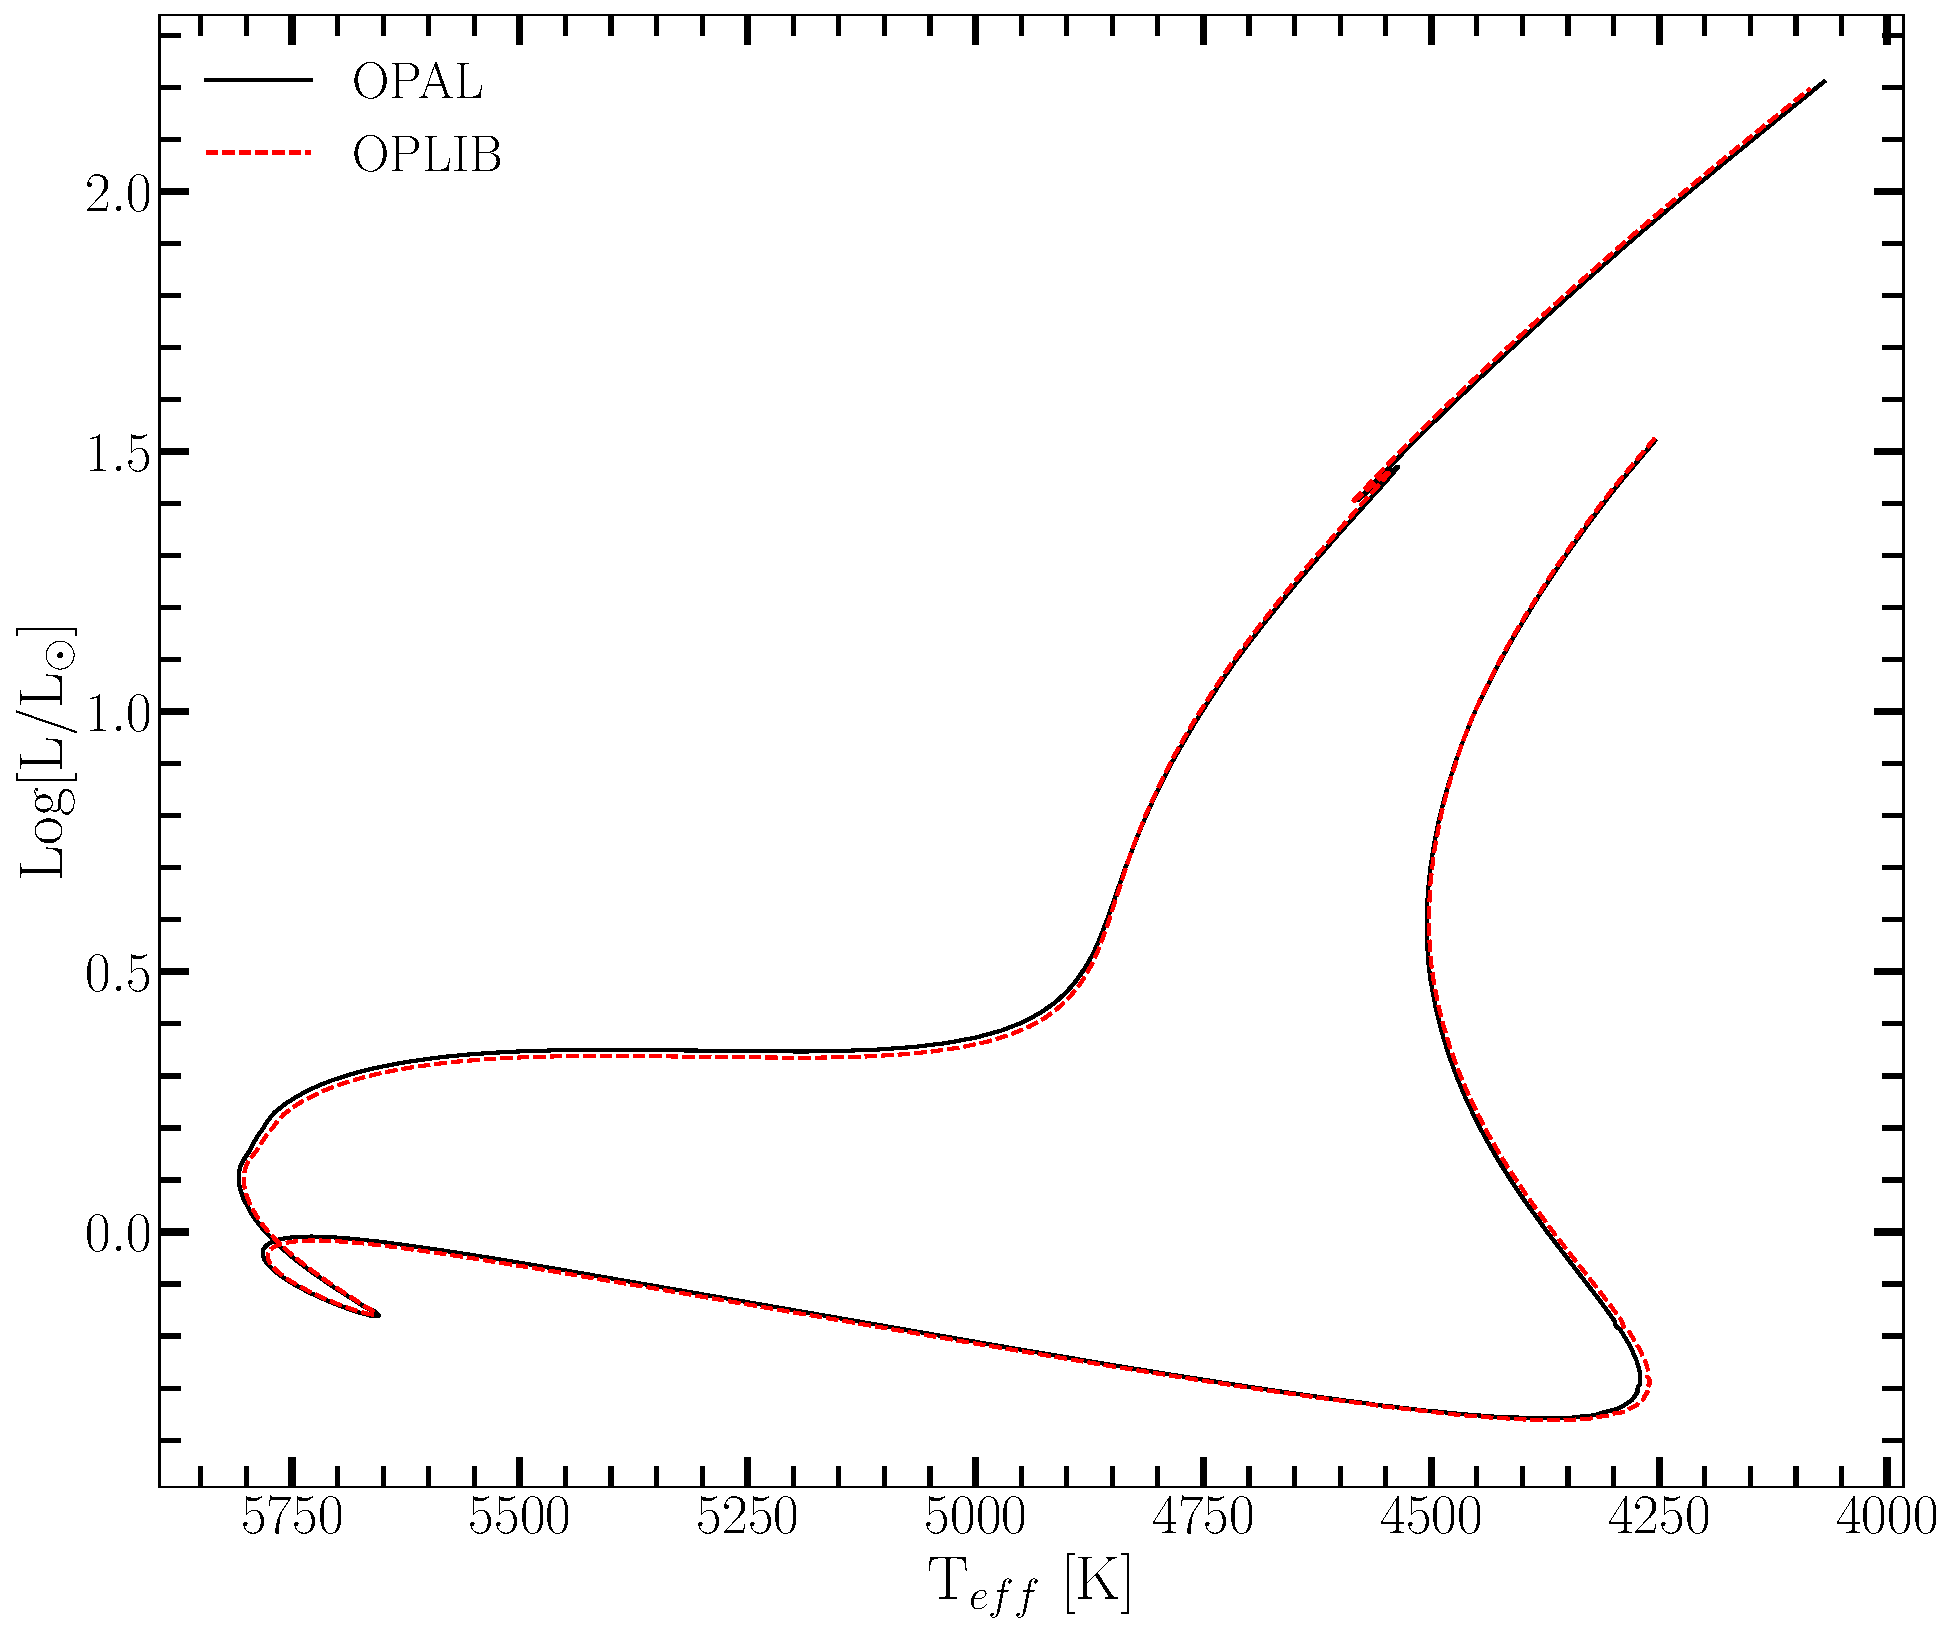
\includegraphics[width=0.28\textwidth]{src/Figures/HRDiagramOPALvsOPLIB_SCCM.pdf}
			\end{tikzfigure}

			\tikzpar For $\log(R)=-1.5$, OPAL and OPLIB opacities vary up to
			approximately 2\% when $T\geq10^{6}$ K. We calibrate a solar model
			(above) to confirm that variations of this order do not
			dramatically alter a solar model's evolutionary path.


			\tikzpar These small variations may be more impactful for stars at or near
			the convective transition mass. The interior structure, which is
			believed to result in the Jao Gap, of such stars is very sensitive
			to temperature; therefore, small changes in opacity may be more
			impactful than in higher mass models.
	    }

		\block{References}{
			\begin{minipage}[t]{0.75\linewidth}
				{\fontsize{24}{22}\selectfont
				\begin{enumerate}
					\item Dotter, A., Chaboyer, B., Jevremovi ́c, D., et al. 2008, The Astrophysical Journal Supplement Series, 178, 89 
					\item van Saders, J. L., \& Pinsonneault, M. H. 2012, The Astrophysical Journal, 751, 98
					\item Jao, W.-C., Henry, T. J., Gies, D. R., \& Hambly, N. C. 2018, ApJL, 861, L11,
				\end{enumerate}
				}
			\end{minipage}%
			\begin{adjustbox}{valign=t}
			\begin{minipage}[t]{0.25\linewidth}
				\hspace{5mm}
				
\includegraphics[scale=0.65]{src/QR.pdf}
			\end{minipage}
			\end{adjustbox}
			{\fontsize{24}{22}\selectfont
			\begin{enumerate}
				 \setcounter{enumi}{3}
				 \item Colgan, J., Kilcrease, D. P., Magee, N. H., et al. 2016, in APS Meeting Abstracts, Vol. 2016, APS Division of Atomic, Molecular and Optical Physics Meeting Abstracts, D1.008
			\end{enumerate}
			}
		}
	

	    \column{0.66}
		\block{Modeling the Gap}{\fontsize{38}{45}\selectfont
			A theoretical explanation for the Jao Gap comes from
			van Saders \& Pinsonneault 2012, who propose that in a star directly above the
			transition mass, due to asymmetric production and destruction of
			He$^{3}$ during the proton-proton I chain (ppI), periodic
			luminosity variations can be induced. This is known
			as convective-kissing instabilitie.
			
	        \begin{tikzfigure}[Internal Evolution of a star experiencing convective kissing instabilities. The shaded region shows the where in the model radiative transport dominates.]
	        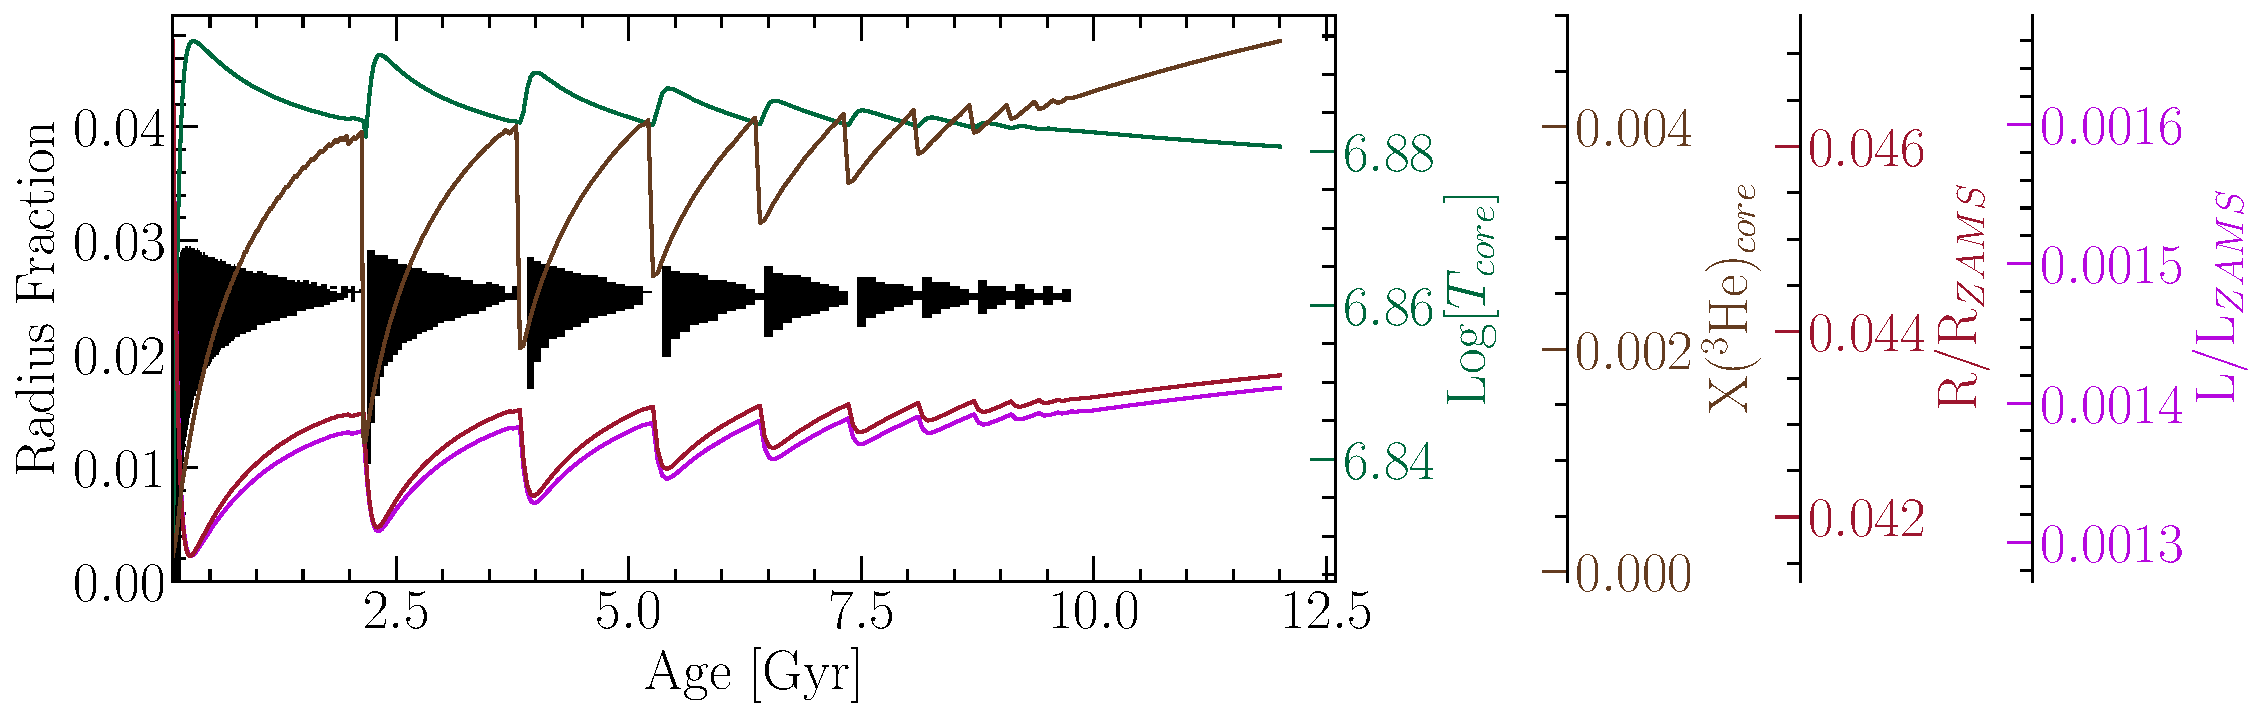
\includegraphics[width=0.6\textwidth]{src/Figures/NBFigs/Kippenhan.pdf}
	        \end{tikzfigure}

			We evolve a set of models with very finely spaced masses (dM=0.002
			M$_{\odot}$) using DSEP (Dotter et al. 2008). These models are
			transformed into Gaia DR2 bolometric magnitudes. Photometric and
			astrometric uncertainties are introduced into the sampled
			populations using empirically calibrated relations between Gaia DR2
			parameters.

			\begin{tikzfigure}[Population synthethis results derived from models evolved using OPAL high temperature opacity tables and models evolved using OPLIB high temperature opacity tables. A gaussian kernel density estimator is displayed on top of the points. Note how the Jao gap is visible in both but at a different $M_{G}$.]
	        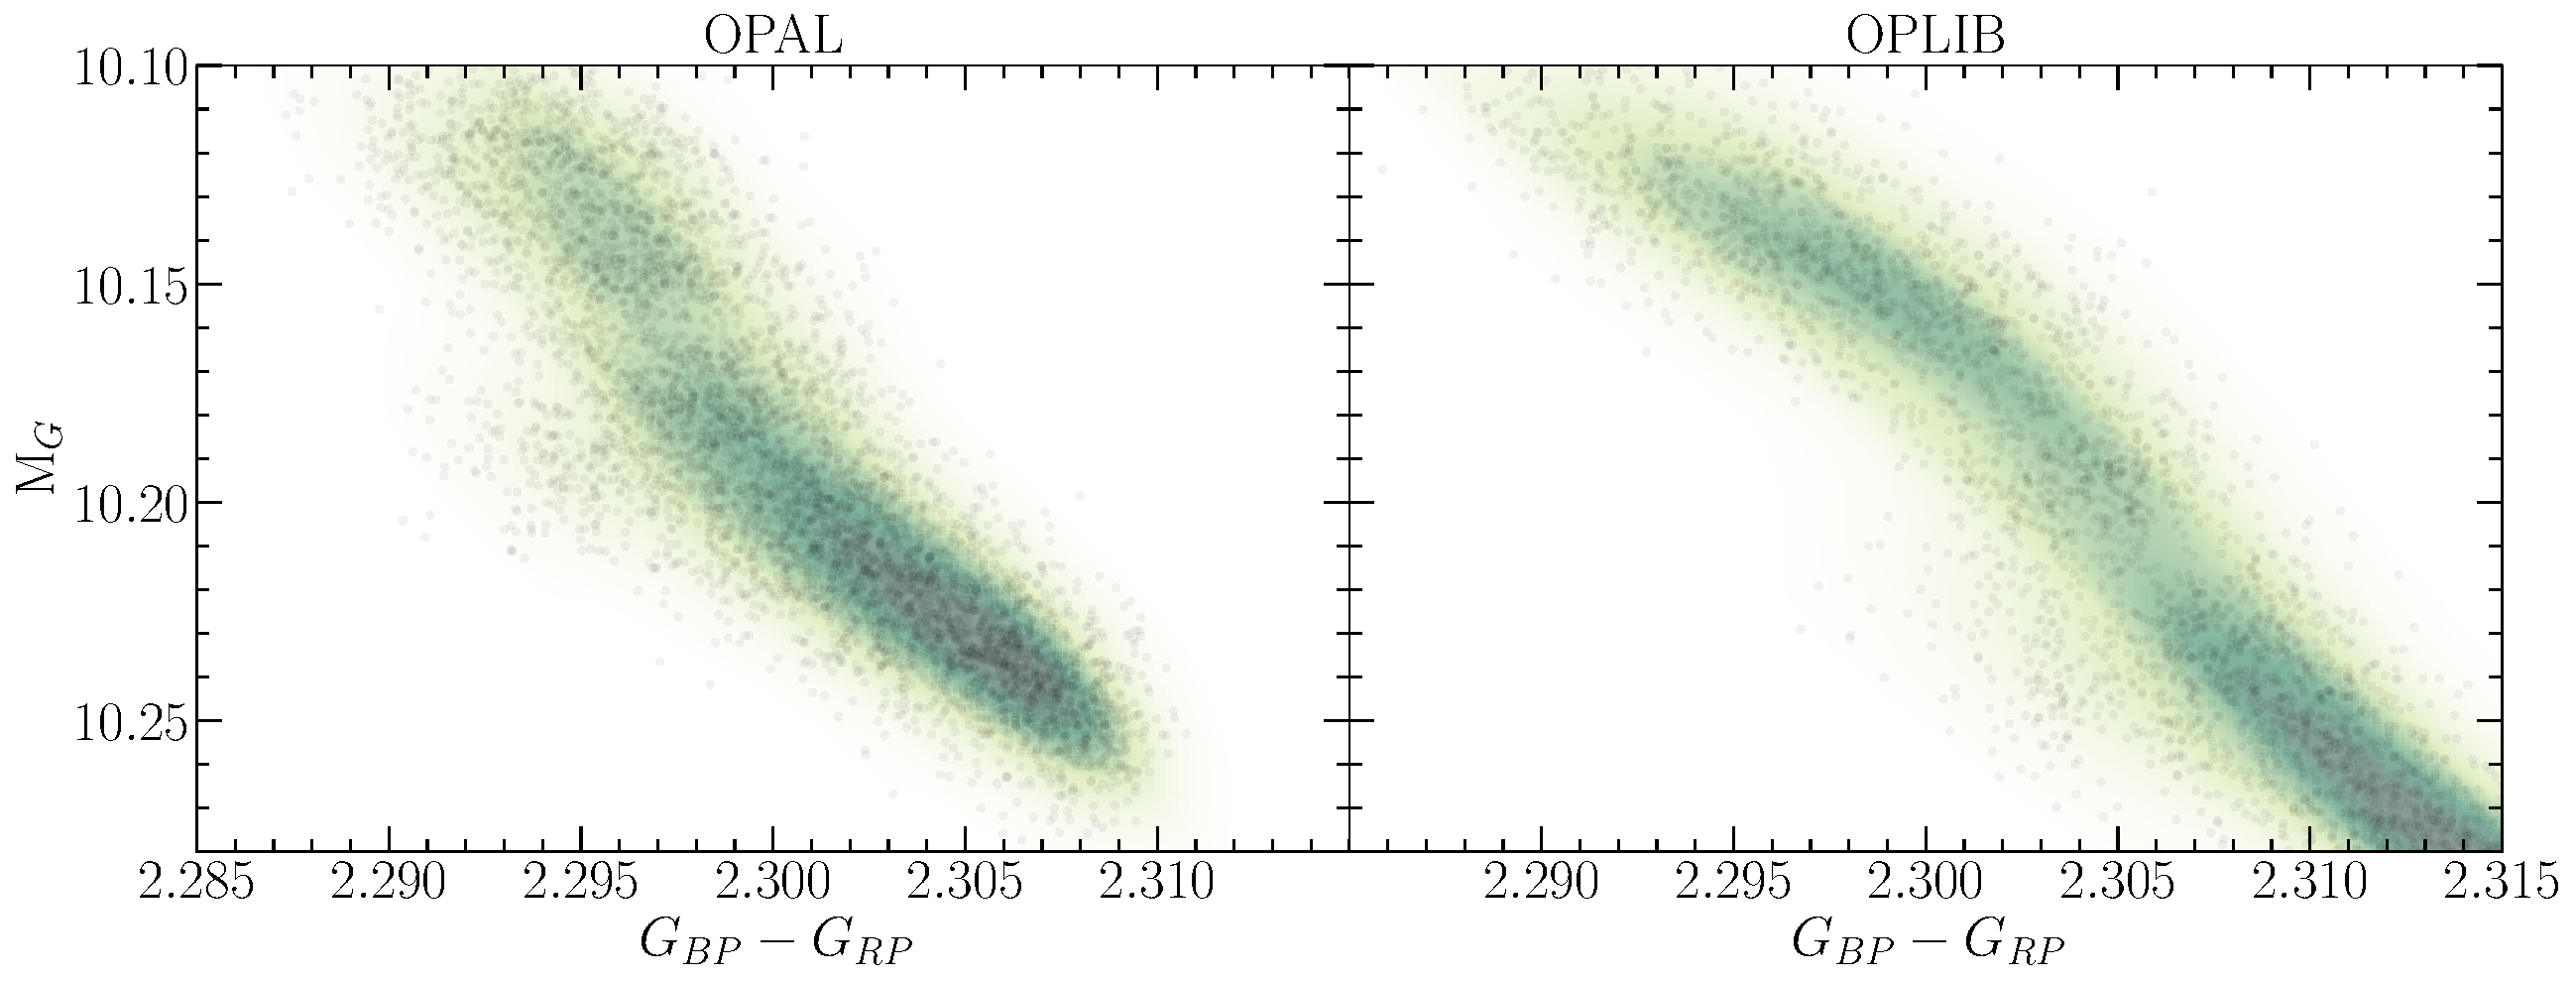
\includegraphics[scale=1]{src/Figures/NBFigs/OPALOPLIB_popsynth_comp_clampedTime.pdf}
	        \end{tikzfigure}

			\vspace{-2cm}
	    }
		\block{Locating the Gap}{\fontsize{38}{45}\selectfont
			\begin{minipage}[t]{0.33\linewidth}
				We locate the Jao Gap using troughs in the number density of
				points along the magnitude axis. Because that density function
				tends to be noisy we run a butter low-pass filter over it
				before selecting all peaks with a prominence greater than 0.1
				as potential Jao Gap locations. 
			\end{minipage}%
			\begin{adjustbox}{valign=t}
			\begin{minipage}[t]{0.66\linewidth}
				\begin{tikzfigure}[We locate the Jao Gap when using OPAL opacity tables at $M_{G} \sim 10.16$ mag]
					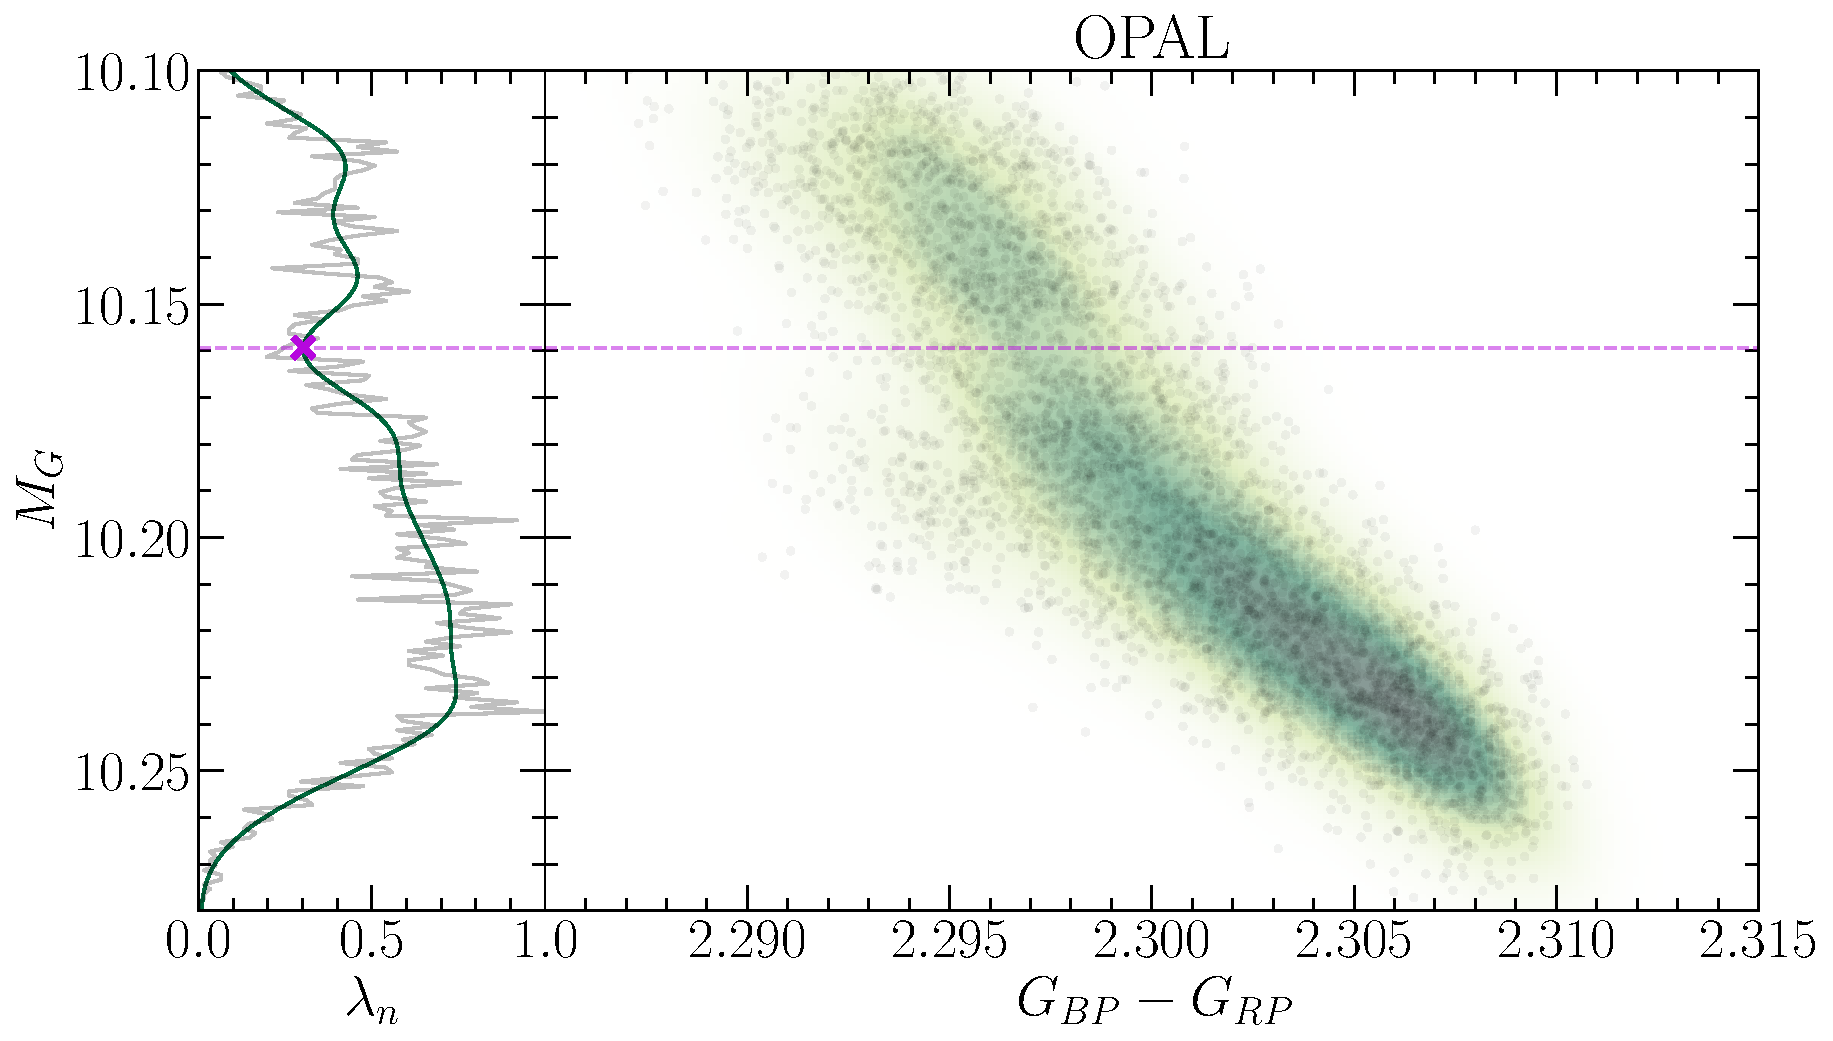
\includegraphics[scale=1]{src/Figures/NBFigs/OPAL_Jao_locator.pdf}
				\end{tikzfigure}
			\end{minipage}
			\end{adjustbox}

			\begin{adjustbox}{valign=t}
			\begin{minipage}[t]{0.66\linewidth}
				\begin{tikzfigure}[Both Jao Gap locations are dimmer than OPAL. This is in line with the slightly lower opacity in OPLIB.]
					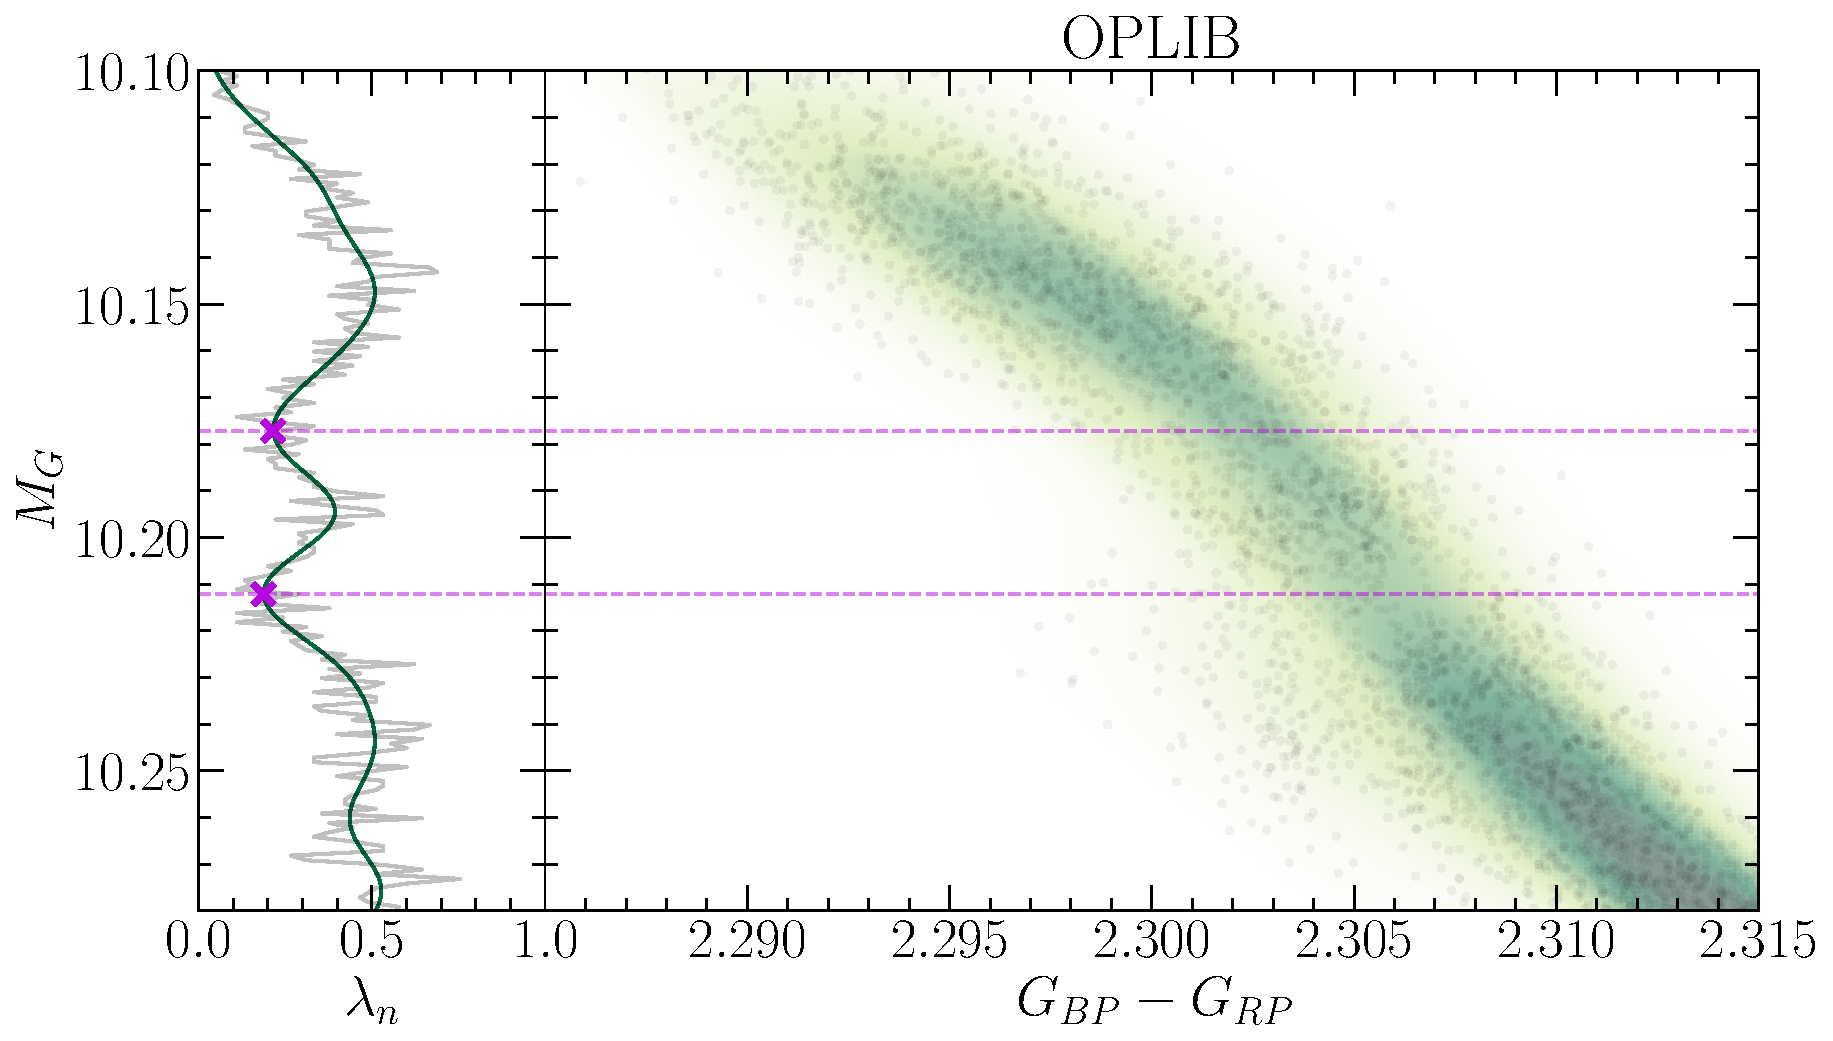
\includegraphics[scale=1]{src/Figures/NBFigs/OPLIB_Jao_locator.pdf}
				\end{tikzfigure}
			\end{minipage}
			\end{adjustbox}
			\begin{minipage}[t]{0.33\linewidth}

			\begin{tikztable}[Identified Jao Gap Locations]
				\centering
				\begin{tabular}{l | r r}
					\hline
					peak & $M_{G}$ & Prominence \\
					\hline
					\hline
					OPAL$_{1}$ & 10.15933 & 0.15671\\
					OPLIB$_{1}$ & 10.17718 & 0.17795 \\
					OPLIB$_{2}$ & 10.21218 & 0.32097 \\
				\end{tabular}
			\end{tikztable}

			{\begin{center}
				\bf{\color{Dgreen}\large Acknowledgments}
			\end{center}}
			{
			\fontsize{23}{20}\selectfont
			We acknowledge the support of an NASA grant (No.
			80NSSC18K0634). Additionally, we would like to thank James
			Colgan for his assistance with the OPLIB opacity tables. We
			would also like to thank Aaron Dotter and Elisabeth Newton.
			}




			\end{minipage}%

			% \column{0.33}
			% \begin{tikzfigure}[Test]
			% 	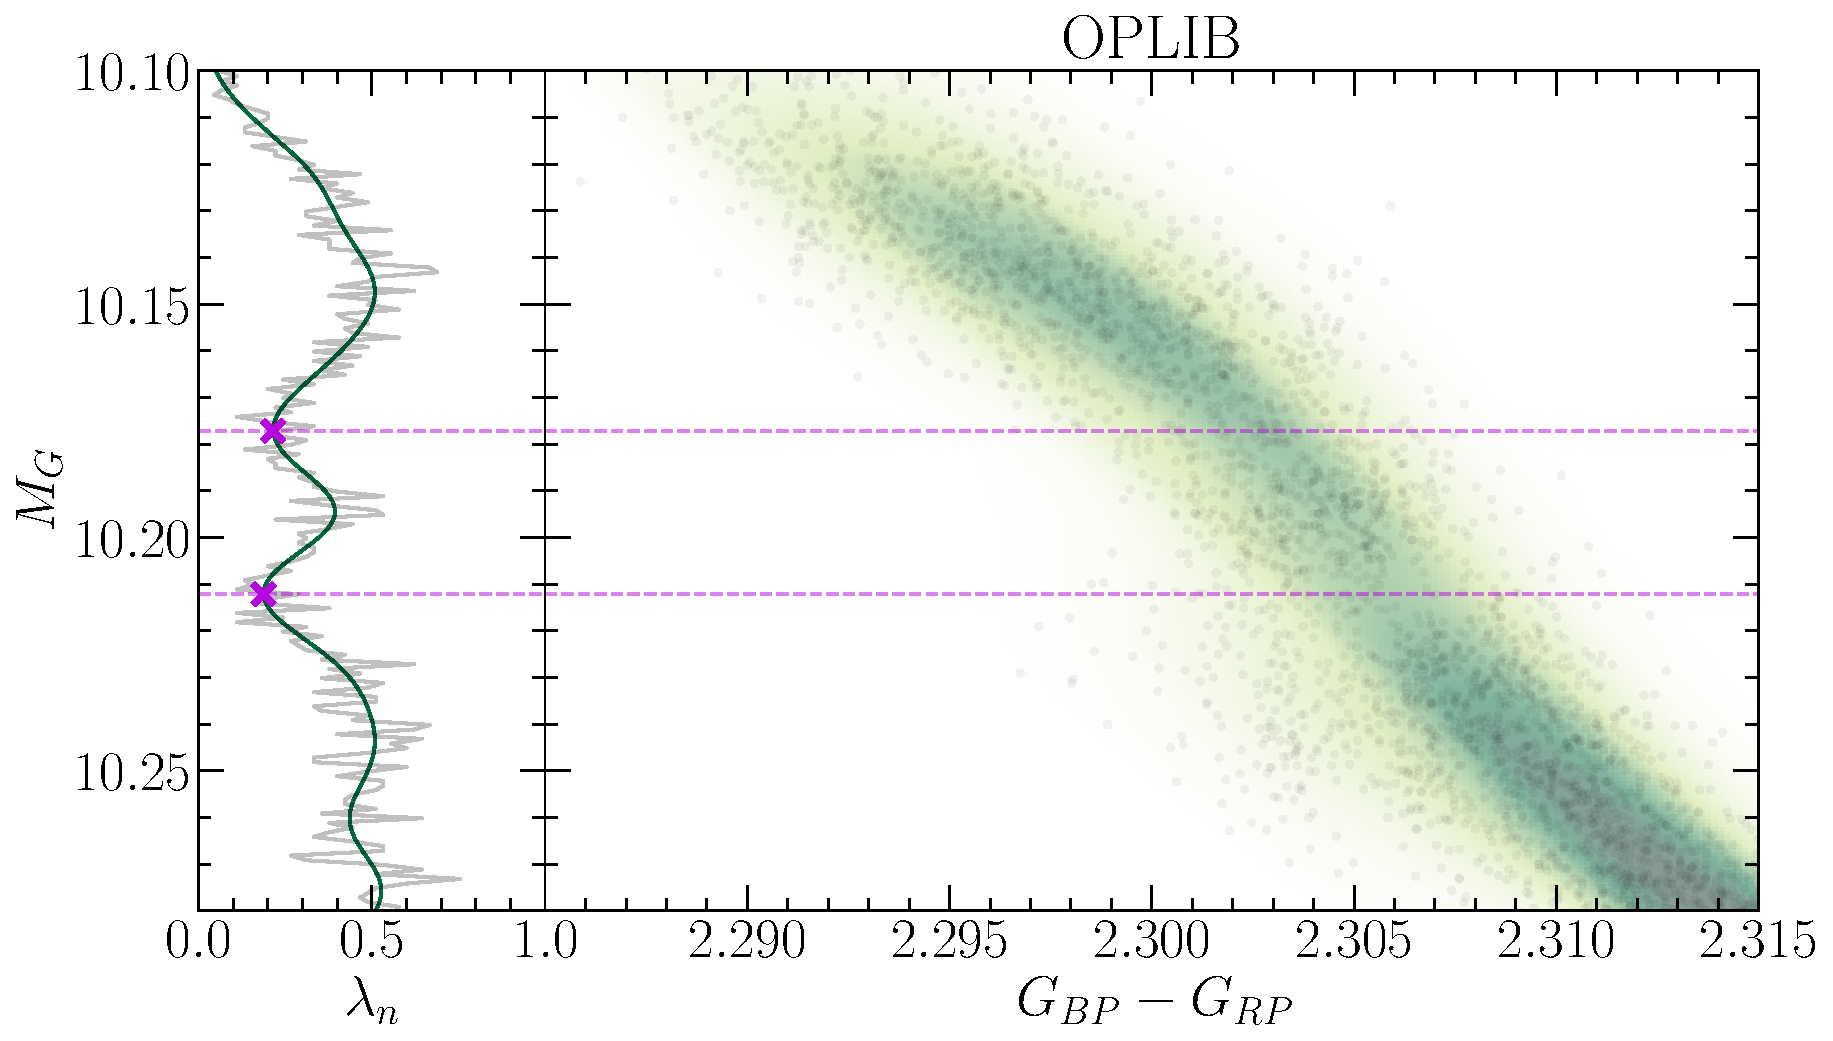
\includegraphics[scale=0.4]{src/Figures/NBFigs/OPLIB_Jao_locator.pdf}
			% 	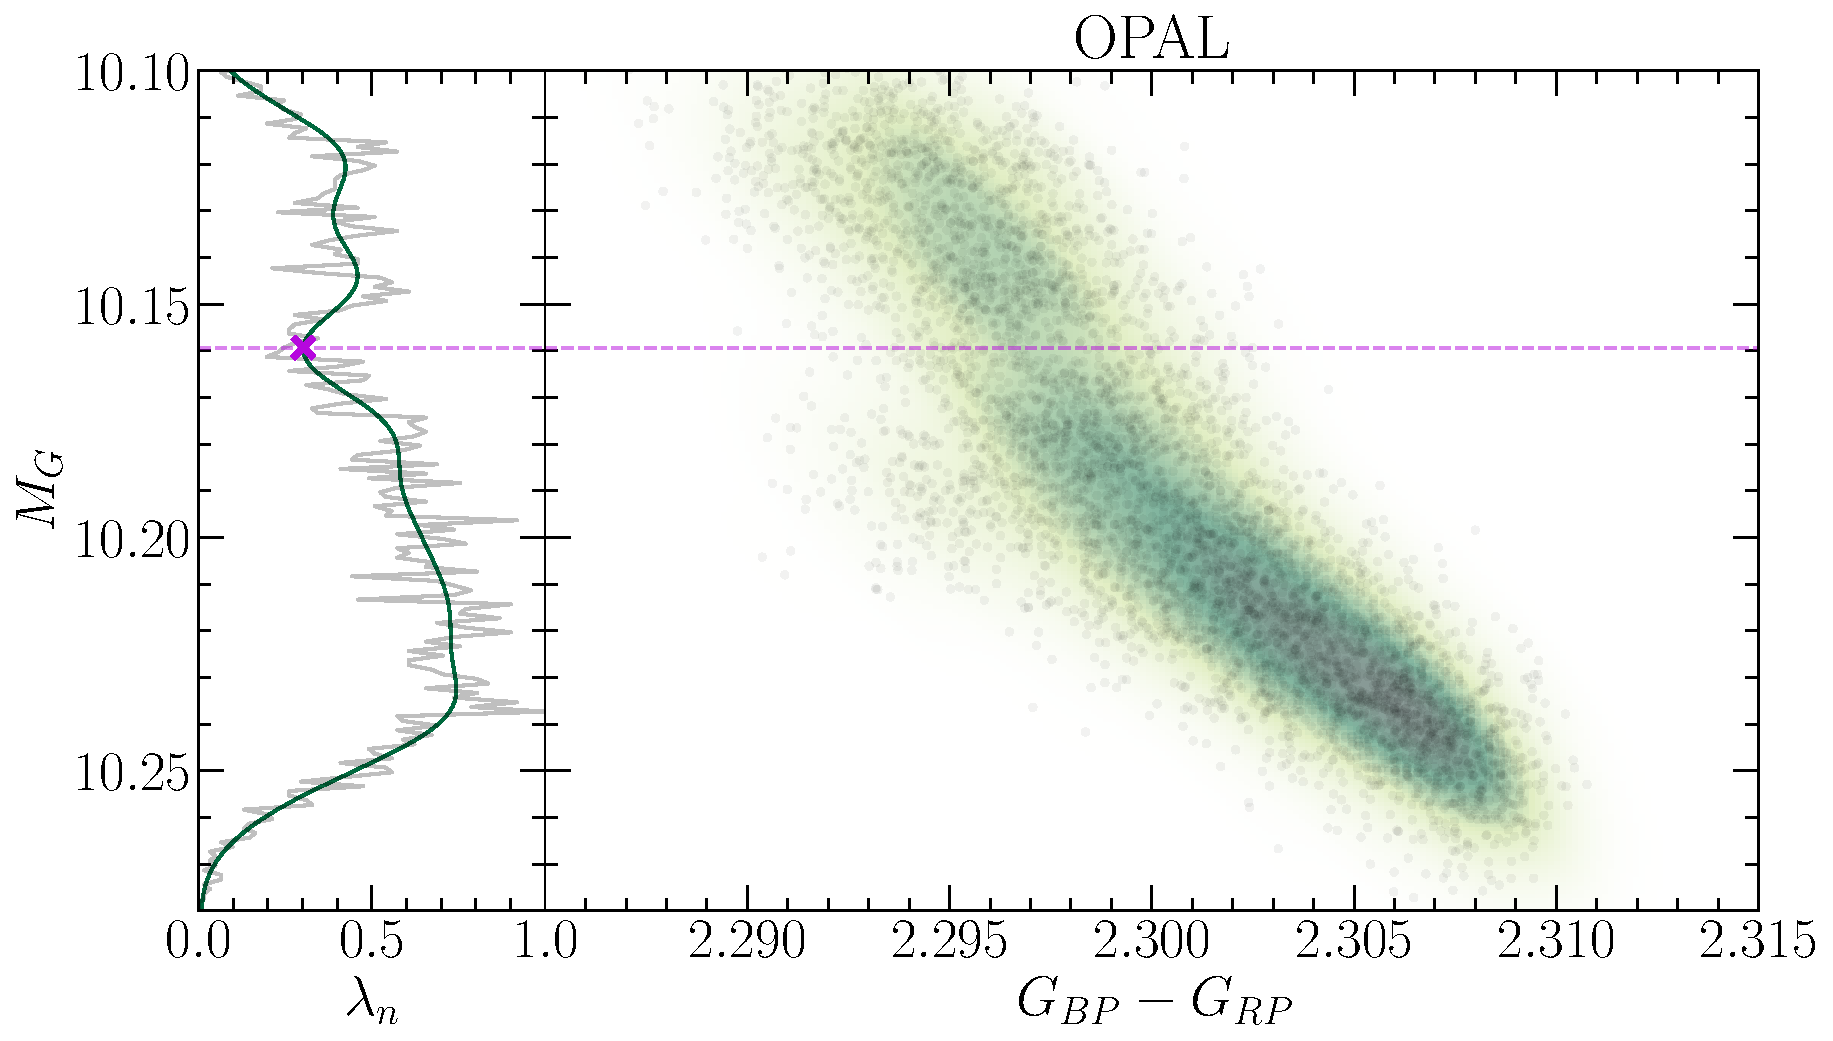
\includegraphics[scale=0.4]{src/Figures/NBFigs/OPAL_Jao_locator.pdf}
			% \end{tikzfigure}
            %
			% \column{0.33}
			% Test Text

		}

		% \column{0.25}
        %
		% \block{Population Synthethis}{
		% 	We 
        %
		% }
        %
	    % \block{{Acknowledgments}}{
	    %     {\fontsize{20}{25}\selectfont
		% 		This research has made use of NASA's astrophysical data system
		% 		(ADS). We acknowledge the support of an NASA grant (No.
		% 		80NSSC18K0634). Additionally, we would like to thank James
		% 		Colgan for his assistance with the OPLIB opacity tables. We
		% 		would like to thank Aaron Dotter, and Elisabeth Newton for
		% 		their assistance. Finally, we thank our colleagues and peers in
		% 		for their continuing and appreciated support.
        %         
        %         
        %     \vspace{-2cm}
        %     }}
        % \block{References}{
        % {\fontsize{20}{25}\selectfont
        %     \begin{enumerate}
        %         \item U. Heber. Hot Subluminous Stars. Publications of the Astronomical Society of the Pacific, 128(8):082001, August 2016. 10.1088/1538-3873/128/966/082001.
        %      \end{enumerate}
        %  }
        % }
	\end{columns}
\end{document}
